%------------Ejercicio 1---------------------------------------

\begin{question}
    Hallar $a \in \mathbb{R}$ positivo tal que el volumen encerrado por las superficies 
    $z = \sqrt{x^2+y^2}$ y $z = a \left( x^2+y^2 \right)$ sea igual a $\frac{\pi}{6}$.
\end{question}

%------------Ejercicio 2---------------------------------------

\begin{question}
    Sea $S$ la superficie parametrizada por $\boldsymbol{\Sigma}: \left[-2,1\right] \times \left[0,1\right] \rightarrow \mathbb{R}^3$ tal que 
    $\boldsymbol{\Sigma}(u,v) = (u+v,u-2v,u^2+v^2)$. Hallar las ecuaciones de todos los planos tangentes 
    a $S$ que resulten paralelos al plano $x+y+z=0$.
\end{question}

%------------Ejercicio 3---------------------------------------

\begin{question}
    Sea $C$ una curva simple parametrizada por $\boldsymbol{\sigma}:[0,1] \rightarrow \mathbb{R}^3$ tal que 
    $\boldsymbol{\sigma}(0)=\boldsymbol{\sigma}(1)$  y sea el campo $\boldsymbol{F}(x,y,z) = (y^2-2xz+g(x),2xy+z^3-g(y),3yz^2-x^2)$
    con $g:\mathbb{R}\rightarrow \mathbb{R}$ una función de clase $C^1$. Calcular $\int_{C}F \cdot ds$.
\end{question}


%------------Ejercicio 4---------------------------------------

\begin{question}
    Sea $C$ la curva simple formada por los segmentos $y=0$ si $x \in [1,2]$ y 
    $x=0$ si $y \in [1,2]$, y por las curvas $y=\sqrt{4-x^2}$ y $y=\sqrt{1-x^2}$ ambas en el primer
    cuadrante. Calcular, indicando la orientación elegida,
    \begin{equation*}
        \int_{C} \frac{x}{x^2+y^2}dx - \frac{y}{x^2+y^2}dy.
    \end{equation*}
\end{question}

%------------Solucion 1---------------------------------------
\newpage
\begin{solution}
    Primero, es útil reconocer qué superficies son las que encierran el volumen.
    \begin{center}
        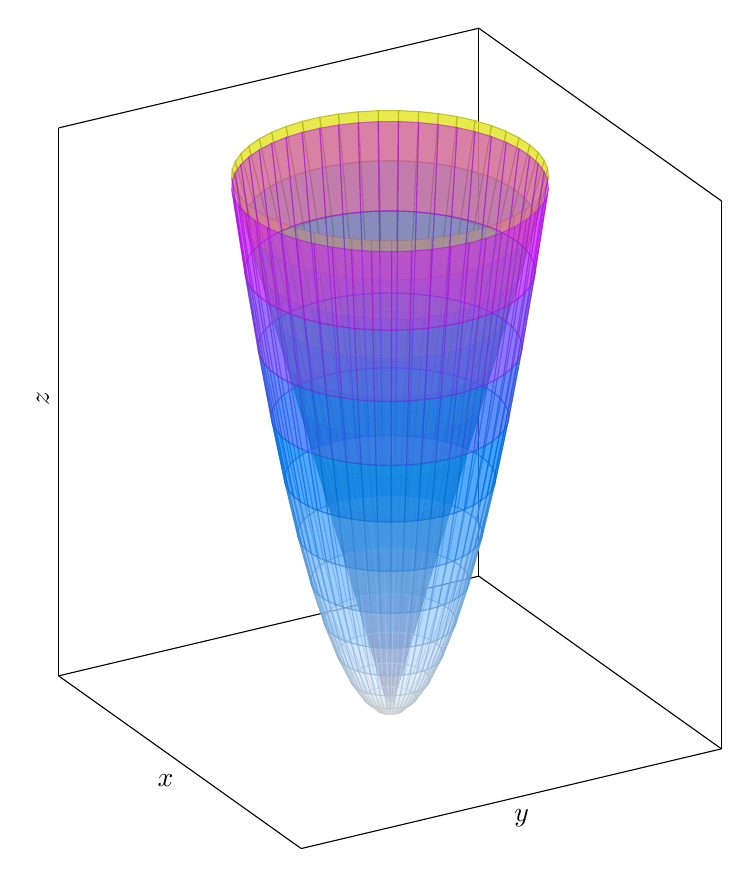
\begin{tikzpicture}
            \begin{axis}[
                    view={60}{20},
                    xlabel=$x$,
                    ylabel=$y$,
                    zlabel=$z$,
                    xmin=-1.5,
                    ymin=-1.5,
                    zmin=0,
                    xmax=1.5,
                    ymax=1.5,
                    zmax=1,
                    samples=50,
                    width=10cm,
                    height=12cm,
                    ticks=none
                ]
                \addplot3 [surf, opacity=0.8, draw=none, restrict z to domain=0:1,
                data cs=polar, domain=0:360, y domain=0:4, colormap/viridis] {max(y,y^2)};

                
                \addplot3 [surf, opacity=0.5, draw=none, restrict z to domain=0:1,
                    data cs=polar, domain=0:360, y domain=0:4, colormap/cool] {min(y,y^2)};

                
            \end{axis}
        \end{tikzpicture}
    \end{center}
    El volumen encerrado $\Omega$, entonces, es aquel entre el semicono $S_{1}:z = \sqrt{x^2+y^2}$ y el paraboloide elíptico $S_{2}:z= a(x^2+y^2)$. 
    La intersección de ambas superficies sucede, arbitrariamente, para $(x,y,z)=(0,0,0)$, y, con $z \neq 0$,  para los puntos:
    \begin{align*}
        a(x^2+y^2)&=\sqrt{x^2+y^2}\\
        a\sqrt{x^2+y^2}&=1\\
        x^2+y^2&=\frac{1}{a} \quad , \quad a\neq 0
    \end{align*}
    Puesto que tales puntos pertenecen a ambas superficies, la curva intersección es 
    \begin{equation*}
        C=\left\{(x,y,z)\in\Rn{3}:x^2+y^2=\frac{1}{a} \land z=\frac{1}{a}\right\}.    
    \end{equation*}
    Así, se puede representar el volumen en coordenadas cartesianas como 
    \begin{equation*}
        \Omega=\left\{ (x,y,z) \in \mathbb{R}^3 : a(x^2+y^2)\leq z \leq \sqrt{x^2+y^2}, 0\leq \sqrt{x^2+y^2}\leq\frac{1}{a} \right\}.
    \end{equation*} 
    Sin embargo, la representación elemental del conjunto es más conveniente en coordenadas cilíndricas. 
    \[\begin{dcases}
            x=r\sen\phi \\
            y=y         \\
            z=r\cos\phi
        \end{dcases}\]
    De tal forma que resulta 
    \begin{equation*}
        \Omega=\left\{ (\rho,\phi,z) \in \mathbb{R}^3 : 0 \leq \phi < 2\pi \land  a\rho^2\leq z \leq \rho \land 0\leq\rho\leq\frac{1}{a}\right\}.    
    \end{equation*}
    Ahora, queda encontrar cual es ese volumen encerrado, realizando la integral, en coordenadas cilíndricas:
    \begin{align*}
        \text{Vol}(\Omega)&=\iiint_{\Omega}dV\\
        &=\iiint_{\Omega}dxdydz \\
        &=\iiint_{\Omega}\rho d\phi dz d\rho \\
        &=\int^{\frac{1}{a}}_{0} \int^{\rho}_{a\rho^2} \int^{2\pi}_{0} \rho d\phi dz d\rho \\
        &=\int^{\frac{1}{a}}_{0} \int^{\rho}_{a\rho^2} \rho \left. \phi \right|^{\phi=2\pi}_{\phi=0} dz d\rho \\
        &=2\pi \int^{\frac{1}{a}}_{0} \int^{\rho}_{a\rho^2} \rho dz d\rho \\
        &=2\pi \int^{\frac{1}{a}}_{0} \rho \left.z\right|^{z=\rho}_{z=a\rho^2} d\rho \\
        &=2\pi \int^{\frac{1}{a}}_{0} \left( \rho^2-a\rho^3 \right) d\rho \\
        &=2\pi \left.\left( \frac{\rho^3}{3}-a\frac{\rho^4}{4}\right)\right|^{\rho=\frac{1}{a}}_{\rho=0}\\
        &=2\pi \left(\frac{1}{3a^3}-\frac{1}{4a^3}\right)\\
        \text{Vol}(\Omega)&=\frac{\pi}{6a^3} \quad , \quad a\in \Rn{+}
    \end{align*}
    Luego, para encontrar $a$, la restricción es que el volumen encerrado, es decir, el valor de la integral anterior, sea $\frac{\pi}{6}$.
    \begin{align*}
        \text{Vol}(\Omega)&=\frac{\pi}{6}\\
        \frac{\pi}{6a^3}&=\frac{\pi}{6}\\
        a^3&=1\\
        \therefore a&=1
    \end{align*}

\end{solution}

%------------Solucion 2---------------------------------------

\begin{solution}
Para este ejercicio, la visualización de la superficie es difícil sin usar una herramienta graficadora.
Sin embargo, sabemos que el vector normal al plano tangente punto a punto de la superficie, se calcula, usando la parametrización, como:
\begin{align*}
    \boldsymbol{n_S}(u,v)&=\boldsymbol{\Sigma_{u}}(u,v)\times \boldsymbol{\Sigma_{v}}(u,v)\\
    \boldsymbol{n_S}(u,v)&=(1,1,2u)\times(1,-2,2v)\\
    \boldsymbol{n_S}(u,v)&=(2v+4u,2u-2v,-3)
\end{align*}
Para que un plano tangente sea paralelo al plano $x+y+z=0$, sus vectores normales deben ser paralelos. El vector normal al plano anterior, $\boldsymbol{n_{P}}$, es:
\begin{equation*}
    \boldsymbol{n_{P}}\cdot \left(\boldsymbol{x}-\boldsymbol{x_{0}}\right) = 0
\end{equation*}
Con $x_0$ un punto perteneciente al plano. En este caso, tomando $x_0=(0,0,0)$:
\begin{equation*}
    \boldsymbol{n_{P}}\cdot (x,y,z) = 0 = x+y+z \quad \Rightarrow \quad \boldsymbol{n_{P}}=(1,1,1)
\end{equation*}
Ahora, para pedir que $\boldsymbol{n_{P}} \parallel \boldsymbol{n_{S}}$, es equivalente pedir, para un $k\in\R-\{0\}$:
\begin{align*}
    \boldsymbol{n_{S}} &= k \cdot \boldsymbol{n_{P}}\\
    (2v+4u,2u-2v,-3)&= k(1,1,1)
\end{align*}
Lo que resulta en un sistema de 3 ecuaciones con 3 incógnitas.
\[\begin{dcases}
            k = (4u+2v) \\
            k = (2u-2v)         \\
            k = -3
        \end{dcases}\]
De la tercera ecuación se obtiene $k=-3$, y de sumar la primera y la segunda, reemplazando este valor anterior:
\begin{align*}
    2(-3)&=6u\\
    -6&=6u\\
    \Rightarrow u&=-1
\end{align*}
Reemplazando en cualquiera de las dos primeras ecuaciones, se obtiene la solución al sistema con $\left\{u=-1 \land v=\frac{1}{2}\right\}$. 
Entonces, existe un único punto cuyo plano tangente es paralelo al plano $x+y+z=0$, que es 
\begin{equation*}
    (x,y,z)=\boldsymbol{\Sigma}\left(-1,\frac{1}{2}\right)=\left(-\frac{1}{2},-2,\frac{5}{4}\right).    
\end{equation*}

La ecuación del plano tangente de este punto sobre la curva $S$ es:
\begin{align*}
    \boldsymbol{n_{S}}\left(-1,\frac{1}{2}\right)\cdot \left((x,y,z)-\left(-\frac{1}{2},-2,\frac{5}{4}\right)\right) &= 0 \\
    (-3)(1,1,1)\cdot \left((x,y,z)-\left(-\frac{1}{2},-2,\frac{5}{4}\right)\right) &= 0\\
    (1,1,1)\cdot \left((x,y,z)-\left(-\frac{1}{2},-2,\frac{5}{4}\right)\right) &= 0
\end{align*}
\begin{equation}
    \therefore \quad \Pi : \left(x+\frac{1}{2}\right)+(y+2)+\left(z-\frac{5}{4}\right)=0
\end{equation}

\end{solution}

%------------Solucion 3---------------------------------------

\begin{solution}
    En principio, no sabemos la expresión de la parametrización de la curva. La única información que tenemos es que es una curva simple y cerrada, puesto que sus valores inicial y final son iguales.
    Sin embargo, tenemos la expresión del campo $\boldsymbol{F}$, cuya integral sobre la curva $C$ hay que calcular. El ejercicio, por lo tanto, apunta a chequar si $\boldsymbol{F}$ es un campo conservativo, para que:
    \begin{equation*}
        \oint_{C}\boldsymbol{F}\cdot\boldsymbol{ds}=0
    \end{equation*}
    según el corolario para el teorema de la integral sobre una curva de un campo conservativo.

    Ya que $g \in C^1(\R)$, $\boldsymbol{F}$ queda definida de $\boldsymbol{F}:\Rn{3}\rightarrow\Rn{3}$. Así, con el campo definido en un conjunto simplemente conexo, se puede usar que:
    \begin{equation*}
        \nabla \times \boldsymbol{F} = 0 \Leftrightarrow \boldsymbol{F} \text{ es un campo conservativo}
    \end{equation*}
    Así, se calcula el rotor del campo:
    \begin{align*}
        \nabla \times \boldsymbol{F}(x,y,z) &= \nabla \times (y^2-2xz+g(x),2xy+z^3-g(y),3yz^2-x^2)\\[10pt]
        &=  \renewcommand{\arraystretch}{1.5} \begin{vmatrix}
                \mathbf{i} & \mathbf{j} & \mathbf{k} \\
                \partialx & \partialy & \partialz \\
                y^2-2xz+g(x) & 2xy+z^3-g(y) & 3yz^2-x^2
            \end{vmatrix} \\[10pt]
    &= \renewcommand{\arraystretch}{1.5} \begin{pmatrix}
        \partialy(3yz^2-x^2) - \partialz(2xy+z^3-g(y)) \\
        \partialz(y^2-2xz+g(x)) - \partialx(3yz^2-x^2) \\
        \partialx(2xy+z^3-g(y)) - \partialy(y^2-2xz+g(x))
        \end{pmatrix}\\[10pt]
    &= \left(3z^2-3z^2,-2x+2x,2y-2y\right)\\[10pt]
    \nabla \times \boldsymbol{F}(x,y,z) &= (0,0,0) \Rightarrow \boldsymbol{F} \text{ es un campo conservativo.}
    \end{align*}

    Por lo tanto, con $\boldsymbol{F}$ un campo conservativo, podemos usar el corolario antes mencionado y calcular el valor de la integral sobre la curva $C$, cerrada, en cero.
    \begin{equation*}
       \therefore \oint_{C}\boldsymbol{F}\cdot\boldsymbol{ds}=0
    \end{equation*}
\end{solution}

%------------Solucion 4---------------------------------------

\begin{solution}
    Cabe notar que la integral pedida es equivalente a escribir:
    \begin{equation*}
        \int_{C} \frac{x}{x^2+y^2}dx - \frac{y}{x^2+y^2}dy = \int_{C} \left(\frac{x}{x^2+y^2},\frac{-y}{x^2+y^2}\right)\cdot\boldsymbol{ds}
    \end{equation*}
    Donde la curva $C$ es simple y cerrada, por lo que encierra un área $A$, tal que $\partial A^{+}=C^{+}$, orientada arbitrariamente en sentido antihorario.
    \begin{figure}[H]
        \centering
        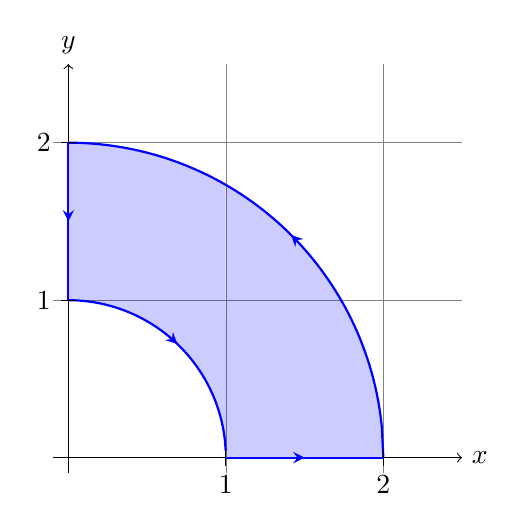
\begin{tikzpicture}[scale=2]

            % Draw the grid
            \draw[very thin,color=gray] (-0.1,-0.1) grid (2.5,2.5);
            
            % Draw the axes
            \draw[->] (-0.1, 0) -- (2.5, 0) node[right] {$x$};
            \draw[->] (0, -0.1) -- (0, 2.5) node[above] {$y$};

            \usetikzlibrary{decorations.markings} % Add the decorations library for arrowheads

            % Define a style for the arrow decoration
            \tikzset{arrow style/.style={postaction={decorate}, 
            decoration={markings, 
                        mark=at position 0.5 with {\arrow{stealth}}}}}
            
            % Draw the curves y=sqrt(4-x^2) and y=sqrt(1-x^2) with color
            \draw[thick, domain=2:0, samples=200, color=blue, arrow style] plot (\x, {sqrt(4-\x*\x)});
            \draw[thick, domain=0:1, samples=200, color=blue, arrow style] plot (\x, {sqrt(1-\x*\x)});
            
            % Draw the lines y=0 for x in [1,2] and x=0 for y in [1,2]
            \draw[thick, color=blue, arrow style] (1,0) -- (2,0);
            \draw[thick, color=blue, arrow style] (0,2) -- (0,1);
            
            % Shade the region between the curves and lines
            \fill[blue, opacity=0.2] (1,0) -- (2,0) 
                -- plot[domain=2:1, samples=100] (\x, {sqrt(4-\x*\x)}) -- cycle;
            \fill[blue, opacity=0.2] plot[domain=0:1,  samples=100] (\x, {sqrt(4-\x*\x)})
                -- plot[domain=1:0, samples=100] (\x, {sqrt(1-\x*\x)}) -- cycle;
            
            % Number the axes
            \foreach \x in {1,2}
            \draw (\x,0.05) -- (\x,-0.05) node[below] {\x};
            \foreach \y in {1,2}
            \draw (0.05,\y) -- (-0.05,\y) node[left] {\y};
            
        \end{tikzpicture}
    \end{figure}
    Puesto que $C$ está orientada antihoraria y encierra una región $A$, simplemente conexa, se puede usar el teorema de Green.
    \begin{equation*}
        \oint_{C^+} \left(\frac{x}{x^2+y^2},\frac{-y}{x^2+y^2}\right)\cdot\boldsymbol{ds} = \iint_{A} \nabla \times \left(\frac{x}{x^2+y^2},-\frac{y}{x^2+y^2}\right)dA
    \end{equation*}
    Tal que el rotor del campo en cuestión se calcula:
    \begin{align*}
        \nabla \times \left(\frac{x}{x^2+y^2},\frac{-y}{x^2+y^2}\right) &= \partialx\left(\frac{-y}{x^2+y^2}\right) - \partialy\left(\frac{x}{x^2+y^2}\right)\\[10pt]
        &= \frac{y\cdot2x}{\left(x^2+y^2\right)^2} - \frac{x\cdot(-2y)}{\left(x^2+y^2\right)^2}\\[10pt]
        &= \frac{4yx}{\left(x^2+y^2\right)^2}
    \end{align*}
    Mientras que la región $A$ puede ser expresada, convenientemente, en coordenadas polares.
    \begin{equation*}
        A=\left\{(\rho,\phi)\in\Rn{2}:0\leq\phi\leq\frac{\pi}{2} \land 1\leq \rho \leq 2\right\}
    \end{equation*}
    Así, la integral se puede resolver en coordenadas polares como:
    \begin{align*}
        \iint_{A} \nabla \times \left(\frac{x}{x^2+y^2},-\frac{y}{x^2+y^2}\right)dA &= \iint_{A} \frac{4yx}{\left(x^2+y^2\right)^2}dxdy\\[10pt]
        &= \iint_{A}\left( \frac{4 \rho \sin{(\phi)} \rho \cos{(\phi)}}{\rho^4}\cdot \rho \right) d\rho d\phi\\[10pt]
        &= \iint_{A}\left( \frac{2 \sin{(2\phi)}}{\rho}\right) d\rho d\phi\\[10pt]
        &= \int^{\frac{\pi}{2}}_{0}\int^{2}_{1}\left( \frac{2 \sin{(2\phi)}}{\rho}\right) d\rho d\phi\\[10pt]
        &= \int^{\frac{\pi}{2}}_{0}\left(2\sin{(2\phi)}\left.\ln(\rho)\right|^{\rho=2}_{\rho=1}\right) d\phi\\[10pt]
        &= \int^{\frac{\pi}{2}}_{0}\left(2\sin{(2\phi)}\ln\left(\frac{2}{1}\right)\right) d\phi\\[10pt]
        &= \ln(2)\cdot 2\left.\left(\frac{-\cos{(2\phi)}}{2}\right)\right|^{\phi=\frac{\pi}{2}}_{\phi=0}\\[10pt]
        &= \ln(2)\cdot 2\\[10pt]
        \Rightarrow \iint_{A} \nabla \times \left(\frac{x}{x^2+y^2},-\frac{y}{x^2+y^2}\right)dA &= 2\ln(2)
    \end{align*}
    Que, volviendo a Green, determina el valor de la integral original.
    \begin{equation*}
         \therefore \int_{C^+} \frac{x}{x^2+y^2}dx - \frac{y}{x^2+y^2}dy = 2\ln(2)
    \end{equation*}
\end{solution}